\apendice{Especificación de diseño}

\section{Introducción}

En este apéndice se presentará aquello referente al diseño de la aplicación. En una primera parte analizaremos los datos con los que trabaja la aplicación y también qué datos exporta. A continuación veremos en profundidad los principales procedimientos que contiene la aplicación y en una última parte, el diseño arquitectónico centrándonos en el código del proyecto.

\section{Diseño de datos}

Para resolver el problema planteado hemos utilizado variables dentro del código que nos permiten guardar todos los datos tanto para resolver como para mostrar sistemas de ecuaciones con restricciones.

\begin{itemize}
    \item \textbf{Formulario tamaño matriz: }el primer requerimiento fue contar con un elemento encargado de definir el tamaño de filas por columnas de nuestra matriz de datos de entrada. Este formulario va a requerir dos únicos valores: marcadores y fuentes.
    
    \item \textbf{Formulario matriz:} matriz con un tamaño definido por los índices del primer formulario, este \textit{FormGroup} que contiene tantos \textit{FormControls} como $marcadores\:x\:fuentes$, tiene un tamaño fijo, pero el usuario puede crear otro nuevo mediante el primer formulario. En el código se encuentra como \textbf{Matrix}
    
    \item \textbf{Formulario mezclas: }formulario de marcadores de las fuentes. En el caso de este formulario su tamaño de marcadores es fijo marcado por el primer formulario y su segundo índice parte de uno y el usuario puede añadir tantas mezclas como quiera. En el código se nombra como \textbf{Results}.
\end{itemize}

\section{Diseño procedimental}

En esta sección recorreremos los principales flujos de la aplicación y veremos las secuencia de operaciones que realizan los componentes entre sí.

\subsubsection{Flujo-01}

En este primer flujo se parte del estado inicial de la aplicación. La ruta por defecto de la aplicación es el componente \textit{"MatrixComponent"} que sería el encargado de resolver el sistema de ecuaciones. Por esa razón el texto escrito en html \textit{<router-outlet>} nos redirige al componente \textit{"MatrixComponent"}. Una vez situados en el punto de partida el usuario rellena el primer formulario con los tamaños de la matriz fuentes, lanzando la función \textit{crearMatrix()}. Como respuesta nos devuelve una matriz de arrays de fuentes y de mezclas a rellenar por el usuario (el usuario puede añadir con un botón tantas mezclas como quiera). Cuando se complete la introducción de datos el usuario pulsa a resolver que lanzará de nuevo una función en \textit{"matrix.component.ts"}, esta función hace tantas iteraciones como mezclas se han configurado y retorna dos arrays: uno de máximo y otro de mínimos por mezcla.

\begin{figure}[h!] 
\centering
    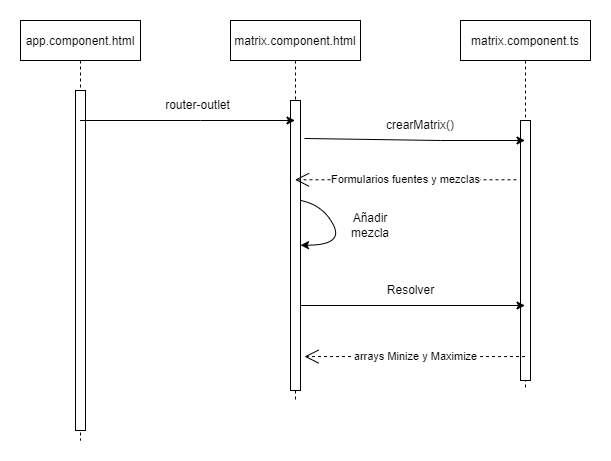
\includegraphics[width=1\textwidth]{img/flujo_01.drawio.png}
\caption{Flujo-01}
\label{fig:flujo_01}
\end{figure}

\newpage
\subsubsection{Flujo-02}

En este segundo flujo partimos del estado donde termino el flujo de la figura \ref{fig:flujo_01}, el cual es justo cuando el usuario visualiza la solución. Justo debajo de la solución se podrían encontrar dos botones ``Exportar problema' y ``Exportar solución''. El primero activa la función \textbf{exportProblem()} que genera un documento con los datos de entrada y llama a un componente de angular encargado de generar el archivo a descargar en el navegador. Este proceso es repetido de la misma forma al pulsar ``Exportar solución'', aunque añadiendo los datos de los arrays solución. Por último el usuario puede hacer click sobre cualquiera de los números de la solución y esto provocara una llamada a la función \textbf{download()} que genera un documento con la resolución de los pasos intermedios y este es descargado en el propio navegador al igual que los documentos anteriores.

\begin{figure}[h!] 
\centering
    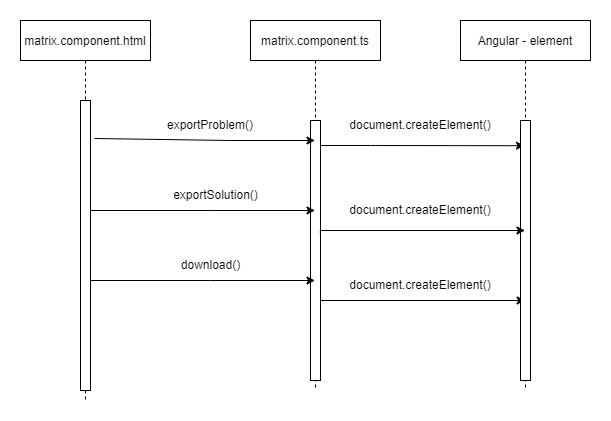
\includegraphics[width=1\textwidth]{img/flujo_02.drawio.png}
\caption{Flujo-02}
\label{fig:flujo_02}
\end{figure}

\subsubsection{Flujo cambio idioma - traducciones}

En este flujo hemos realizado el procedimiento llevado por la aplicación para realizar el cambio de idioma de las traducciones. Partimos de cualquier estado ya que el menú superior siempre está presente en la aplicación. Por tanto en el momento que cambia el select al otro idioma disponible se lanza un evento de cambio \textit{changeLang(event.target())} este evento cambia una variable ubicada en el local storage de la aplicación y toma como valor el seleccionado por el usuario. Esto hace que al realizar las traducciones tome el fichero correspondiente al idioma marcado \textit{assets/i18n/es.json} o \textit{assets/i18n/en.json}. 

\begin{figure}[h!] 
\centering
    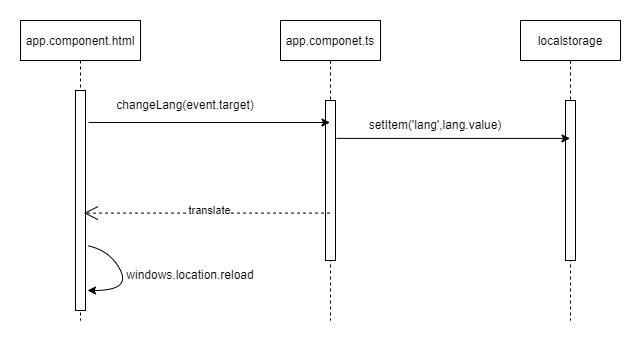
\includegraphics[width=1\textwidth]{img/traducciones.drawio.png}
\caption{Flujo traducciones}
\label{fig:flujo_traduc}
\end{figure}

\newpage
\section{Diseño arquitectónico}

Para realizar la arquitectura funcional de la aplicación se ha utilizado Angular, que una de sus características es que permite la creación de páginas tipo Single Page Application  (SPA). Se ha desarrollado el código siguiendo el patrón de diseño MVVM que divide la estructura del código en dos claras partes modelo y vista. En angular nos encontramos con dos tipos de archivos .ts encargándose de la lógica y las operaciones, y .html junto a .css encargados de la vista. 

El proyecto de angular está dividido en componentes que están formados por:

\begin{itemize}
    \item \textbf{Archivo .ts}: Vendría a ser el ``Modelo'' y contendría los datos a los que se accede desde la vista, además de métodos que modifican esos datos. La propiedad \textit{"two way binding"} hace un enlace bidireccional permitiendo a los componentes de la aplicación compartir datos, permitiendo escuchar eventos y actualizar valores simultáneamente.
    \item \textbf{Archivo .html}: Junto a el archivo .css que aporta los estilos formarían la "Vista" de la aplicación, presentando al usuario los datos en una interfaz fácil de entender.
\end{itemize}

\subsubsection{Servicios}

Un Servicio o \textit{Service} es una clase, comúnmente decorada con el decorador Injector de Angular, que indica que el Servicio puede inyectar otras dependencias de la aplicación, ya sean otros servicios como Http o hacer consultas AJAX.

\subsubsection{Módulos}

Los NgModules son contenedores para un bloque cohesivo de código dedicado al dominio de la aplicación, un flujo de trabajo o importaciones de librerías. Puede contener componentes, proveedores de servicios y otros archivos. Estos modulos se suelen dividir en las mismas partes: \textit{declarations}, \textit{imports}, \textit{exports} y \textit{providers}.



